\documentclass[tikz]{standalone}

\usepackage{pgfplots}

\begin{document}
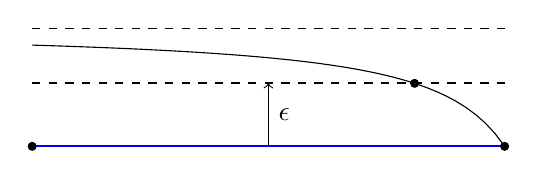
\begin{tikzpicture}

% The plot and asymptote
\draw[domain=-3.0:+3.0,samples=50] plot (\x, {(1 / (\x - 4) + 1) * 1.5});
\draw[dashed] (-3.0, 1.5) -- (+3.0, 1.5);

% The base
\draw[thick, blue] (-3.0, 0) -- (+3.0, 0);
\filldraw (-3.0, 0) circle (0.05);
\filldraw (+3.0, 0) circle (0.05);

% The new line
\draw[thick, dashed] (-3.0, 0.8) -- (+3.0, 0.8);
\filldraw (+1.857, 0.8) circle (0.05);

% Arrow
\draw[->] (0, 0.0) -- (0, 0.8);
\node at (0.2, 0.4) {$\epsilon$};

\end{tikzpicture}
\end{document}
